% Nome do capítulo
\chapter{Metodologia}
% Label para referenciar
\label{cap3}

% Diminuir espaçamento entre título e texto
\vspace{-1.9cm}

O levantamento dos trabalhos relacionados foi feito em sites de bases digitais de artigos científicos, como o \textit{Institute of Electrical and Electronics Engineers} (IEEE), \textit{Association for Computing Machinery} (ACM) e o Portal Capes. O IEEE e o ACM foram escolhidos por serem utilizados com frequência na área de engenharia, já o Portal Capes, por conter periódicos e artigos nacionais. Além disso foram pesquisados trabalhos relacionados em toda a \textit{internet}.

Os trabalhos encontrados nestes portais tratam de modo geral a comparação entre diferentes sistemas de gerenciamento de banco de dados, sendo assim, se torna de extrema relavancia a análise e compreenção das metodologias utilizadas pelos autores, para que possam servir como base para este trabalho. 

Entretanto, nenhum deles abordou uma comparação entre o Sistema de banco de dados atual da SAP em comparação com o novo sistema SAP HANA. 


Para alcançar os objetivos definidos para este trabalho, foi definido o seguinte fluxo de trabalho: 

%\begin{figure}[H]
%  % Alterar espaçamentos antes e depois do caption
%  \setlength{\abovecaptionskip}{0pt}
%  \setlength{\belowcaptionskip}{0pt}
%  % Caption
%  \caption[Fluxo de trabalho]{Fluxo de trabalho}
%  \centering
%  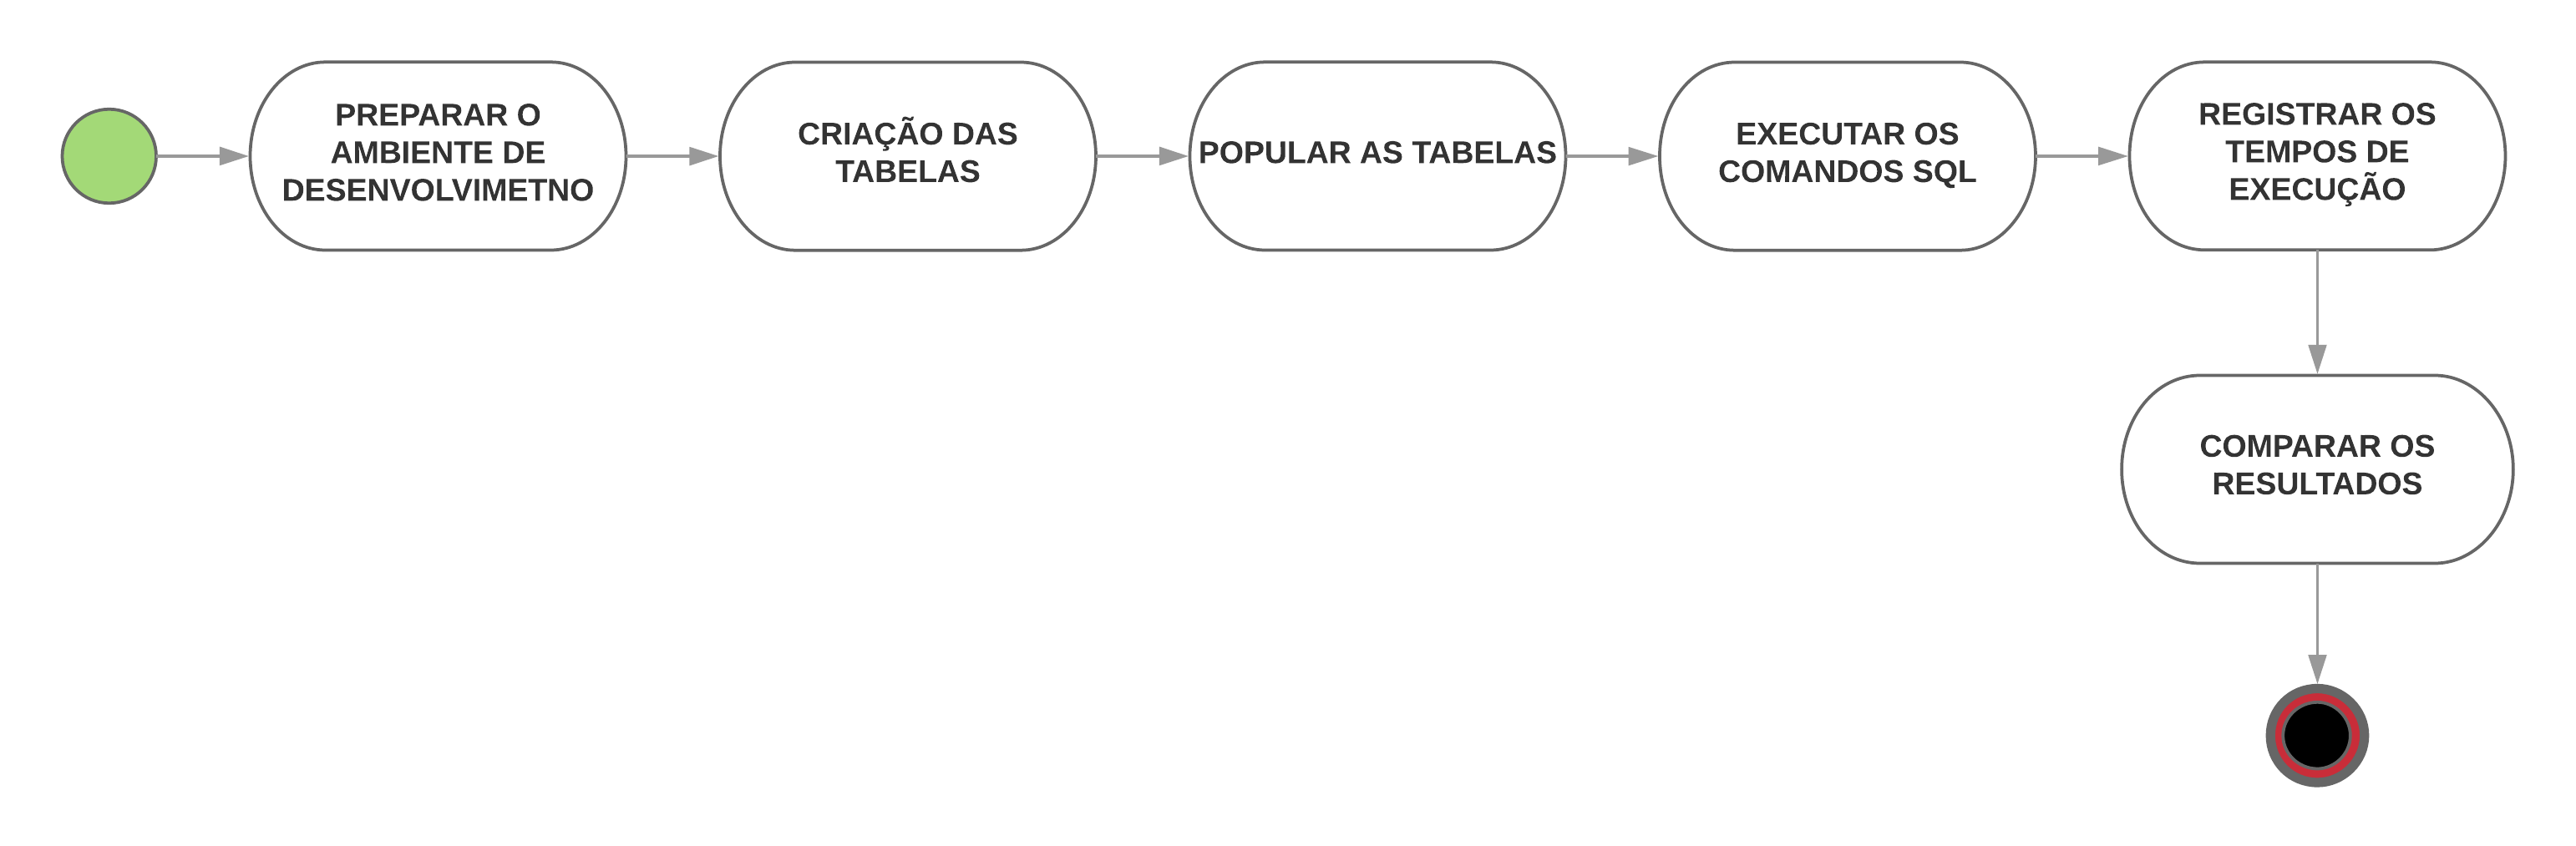
\includegraphics[width=.75\textwidth]{imagem/FLUXO_DEV.png}
%  % Caption centralizada
%  \captionsetup{justification=centering}
%  \captionfont{\small{\textbf{\\Fonte: Autor }}}	
%  \label{fig:4}
%\end{figure}




Como o intuito deste trabalho é realizar alguns testes de performance, entre o banco de dados do SAP ECC e o banco de dados do SAP Hana, realizando algumas consultas de diferentes níveis de dificuldade, atualizações e remoções de dados com o objetivo de medir o tempo de resposta destes SGBDs, se faz necessário detalhar como será o ambiente de testes, o sistema operacional utilizado, hardware e dificuldades encontradas. 

O dados do servidos utilizado estão descritos na tabela 1.
\begin{table}[H]
\centering
\caption{Detalhes do Servidor}
\label{DetalhesServidor}
\begin{tabular}{|l|l|}
\hline
Item                    & Configuração                                                                           \\ \hline
Processador             & Intel(R) Xeon(R) CPU E5-2430 v2 @ 2.50GHz, 2494 Mhz, \\ & 
						  2 Core(s), 2 Logical Processor(s) \\ \hline
Memória RAM             & 8Gb                                                                                    \\ \hline
Disco Rígido            & 150Gb – Disco SATA 10.000   RPM                                                        \\ \hline
Sistema Operacional     & Windows 2008 R2 Standard.                                                              \\ \hline
Banco de dados SAP ECC  & SQL SERVER 2008 R2                                                                     \\ \hline
Banco de dados SAP Hana &                                                                                        \\ \hline
\end{tabular}
\end{table}



%  Este documento foi compilado em ambiente linux (Ubuntu 10.04) usando o programa Kile - an Integrated LaTeX Environment - Version 2.0.85.
%  Para correta formatação os seguintes arquivos do pacote \textit{abntex} devem ser alterados.

 %   \begin{compactitem}
 %     \item[a)] Arquivo abnt.cls

%      No Ubuntu o arquivo fica armazenado em \textit{/usr/share/texmf/tex/latex/abntex}.
%      Comentar a linha 967: Linha comentada para reduzir o espaçamento entre o topo da página e o título.
 %     Alterar a linha 1143: Parâmetro alterado de 30pt para -30pt para reduzir o espaçamento entre o top da página e o título do apêndice.
%      Alterar a linha 985: Parâmetro alterado de 0pt para -30pt para reduzir o espaçamento entre o top da página e o título.
%      Alterar a linha 991: Parâmetro alterado de 45pt para 30pt para reduzir o espaçamento entre o texto e o título.

%      \item[b)] Arquivo acronym.sty

%      No Ubuntu o arquivo fica armazenado em \textit{/usr/share/texmf-texlive/tex/latex/acronym}.
 %     Alterar a linha 225: Inserir o separador -- entre acrônimo/descrição e remover o negrito com o \textit{normalfont}.
      %\item[\protect\AC@hypertarget{#1}{\acsfont{\normalfont{#2}}} --] #3 

 %   \end{compactitem}